%%%%%%%%%%%%%%%%%%%%%%%%%%%%%%%%% Packages/Dokumentart %%%%%%%%%%%%%%%%%%%%%%%%%%%%%%%%%%%%%%%%%%%%%%%%%%%%%%%%%%%%%%%%%%%%%%%%%%%%%%%%%%%%%%%%%%%%%%%%%%%%%%%%%%%%%%%
\documentclass[ a4paper,  % Papierart
 		 %       10pt,    %
   				 12pt,    % Schriftgröße
 			 %  12pt,    %
    			%pdftex,    % PDF Umwandlung
  %  twoside    % 2-seitig
    ] {report}  % Dokumenttyp Bericht
    
\usepackage{geometry} \geometry{a4paper, top=30mm, left=35mm, right=30mm, bottom=30mm, headsep=10mm, footskip=12mm} 
\usepackage[ngerman]{babel}  % Deutsches Sprachpaket/Silbentrennung etc.
\usepackage[utf8]{inputenc}  % verwendeter Codec (für Umlaute)
\usepackage{graphicx}    % für Bilder
\usepackage{cite}    % für bestimmte Zitierfunktionen
\usepackage{url}
\usepackage{nameref}
\usepackage{float}
\newcommand{\myref}[1]{\ref{#1} \textit{\nameref{#1}}}
\newcommand{\fref}[1]{Abbildung \textit{\ref{#1}}}
%\usepackage{hyperref}
\usepackage{acronym}  % für Abkürzungen in Fußnote
\usepackage{caption}    % Um Bildunterschriften zu konfigurieren (mit, ohne erscheinen im Abkürzungsverzeichnis)
\usepackage{setspace}    % für Zeilenabstand
\usepackage{todo}


% Verlinkung zu den Kapiteln im Inhaltsverzeichnis
\usepackage[colorlinks,
pdfpagelabels,
pdfstartview = FitH,
bookmarksopen = true,
bookmarksnumbered = true,
linkcolor = black,
plainpages = false,
hypertexnames = false,
citecolor = black] {hyperref}


\onehalfspacing      % ab hier Zeilenabstand 1,5

\clubpenalty = 10000  
\widowpenalty = 10000  
\displaywidowpenalty = 10000 

%%%%%%%%%%%%%%%%%%%%%%%%%%%%%%%% Kopfzeile %%%%%%%%%%%%%%%%%%%%%%%%%%%%%%%%%%%%%%%%%%%%%%%%%%%%%%%%%%%%%%%%%%%%%%%%%%%%%%%%%%%%%%%%%%%%%%%%%%%%%%%%%%%%%%%%%%%%%%%%%%
\usepackage{fancyhdr}      % Package für Kopfzeile  
\pagestyle{fancy} %eigener Seitenstil
\fancyhf{} %alle Kopf- und Fußzeilenfelder bereinigen
\fancyhead[L]{\leftmark} %Kopfzeile links
\fancyhead[C]{} %zentrierte Kopfzeile
\fancyhead[R]{\rightmark} %Kopfzeile rechts
\renewcommand{\chaptermark}[1]{ \markboth{\thechapter \ #1}{} }
\renewcommand{\sectionmark}[1]{ \markright{\thesection \ #1}{} }

\renewcommand{\headrulewidth}{0.4pt} %obere Trennlinie
\fancyfoot[C]{\thepage} %Seitennummer
\renewcommand{\footrulewidth}{0.4pt} %untere Trennlinie
%\automark[section]{chapter}       % für Anzeigen des Unterkapitels (Standard Überkapitel)
%\clearscrheadfoot \ihead{\headmark}    % ihead links, ohead rechts, chead mitte
%\setheadsepline{0.4pt}        % Linie unter Kopfzeile
%\cfoot[\pagemark]{\pagemark}      % Mitte Fußzeile Seitenzahl (selbe wie mit head (il,o,c))

%%%%%%%%%%%%%%%%%%%%%%%%%%%%%%%%%% Abkürzungen %%%%%%%%%%%%%%%%%%%%%%%%%%%%%%%%%%%%%%%%%%%%%%%%%%%%%%%%%%%%%%%%%%%%%%%%%%%%%%%%%%%%%%%%%%%%%%%%%%%%%%%%%%%%%%%%%%%%%%%
% Persöhnlich
\newcommand{\Autor}{Lukas Essig\\und\\Michael Stahlberger}
\newcommand{\MatrikelNummer}{8898018, 1367912}
\newcommand{\Kursbezeichnung}{TINF11B3}
%Firma
\newcommand{\FirmenName}{Fiducia IT AG }              
\newcommand{\FirmenStadt}{Karlsruhe}              
\newcommand{\FirmenLogoDeckblatt}{
\includegraphics[width=6cm]{Bilder/fiducia.jpg}}  
\newcommand{\dhLogo}{
\includegraphics[width=4cm]{Bilder/dhbw-logo.png}}
%Betreuer
%\newcommand{\BetreuerFirma}{Kay Lützel}
\newcommand{\BetreuerDHBW}{Herr Prof. Hans-Jörg Haubner}
%Art der Arbeit
%\newcommand{\Was}{Praxisbericht}
%\newcommand{\WasErklaerung}{den vorliegenden \Was}
\newcommand{\Was}{Studienarbeit}
\newcommand{\WasErklaerung}{die vorliegende \Was}
%\newcommand{\Was}{Studienarbeit}
%\newcommand{\WasErklaerung}{die vorliegende \Was}
%\newcommand{\Was}{Bachelorarbeit}
%\newcommand{\WasErklaerung}{die vorliegende \Was}
%Deckblatt Infos
\newcommand{\Titel}{Entwicklung einer Gestiksteuerung mittels Kinect für den humanoiden Roboter Nao}
\newcommand{\Dauer}{24 Wochen}
\newcommand{\Abschluss}{Bachelor of Engineering}
\newcommand{\Studiengang}{Informationstechnik}
\newcommand{\AbgabeDatum}{12. Mai 2014}

\begin{document}   %%%%%%%%%%%%%%%%%%%%%%%%%%%%%%%%%%%%%%%%%%%%%%%%%%%%%%%%%%%%%%%%%%%%%%%%%%%%%%%%%%%%%%%%%%%%%%%%%%%%%%%%%%%%%%%%%%%%%%%%%%%%%%%%%%%%%%%%%%%%%%%%%%%%

%%%%%%%%%%%%%%%%%%%%%%%%%%%%%%%%%% Titelseite %%%%%%%%%%%%%%%%%%%%%%%%%%%%%%%%%%%%%%%%%%%%%%%%%%%%%%%%%%%%%%%%%%%%%%%%%%%%%%%%%%%%%%%%%%%%%%%%%%%%%%%%%%%%%%%%%%%%%%%%%
\begin{singlespace}              % Zeilenabstand für Titelseite verringern
\begin{titlepage}
\begin{center}                % Referenzpunkt Seitenmitte
\vspace*{-2cm}                % 2 cm nach Links Platz lassen
\FirmenLogoDeckblatt\hfill
\includegraphics[width=4cm]{Bilder/dhbw-logo}\\[2cm] % Firmenlogo platzieren

{\huge\Titel}\\[2cm]              % \Huge, \Large, \large sind versch. Schriftgrößen \bfseries ist Fett gedruckt
{\Huge\scshape \Was}\\[2cm]            % [] Inhalt ist Abstand zur nächsten Zeile
{\large f\"ur die Pr\"ufung zum}\\[0.5cm]
{\Large \Abschluss}\\[0.5cm]
{\large des Studienganges \Studiengang}\\[0.5cm]
{\large an der}\\[0.5cm]
{\large Dualen Hochschule Baden-W\"urttemberg Karlsruhe}\\[0.5cm]
{\large von}\\[0.5cm]
{\large\bfseries \Autor}\\[1cm]
{\large Abgabedatum \AbgabeDatum}
\vfill                  % ermöglicht es unterhalb der Seitengrenze zu schreiben
\end{center}                % Referenzpunkt Mitte beenden

\begin{tabular}{l@{\hspace{2cm}}l}          % Beginn Tabelle mit einer Spalte nach der 2cm Platz gelassen wird bevor die nächste beginnt
Bearbeitungszeitraum           & \Dauer       \\
Matrikelnummer                   & \MatrikelNummer    \\
Kurs               & \Kursbezeichnung    \\
Ausbildungsfirma   & \FirmenName  \FirmenStadt      \\
Betreuer  & \BetreuerDHBW    \\
\end{tabular}                % Tabelle abschließen
\end{titlepage}
\end{singlespace}                % Titelseite abschließen
%%%%%%%%%%%%%%%%%%%%%%%%%%%%%%%%%%%%%%%%%%%%%%%%%%%%%%%%%%%%%%%%%%%%%%%%%%%%%%%%%%%%%%%%%%%%%%%%%%%%%%%%%%%%%%%%%%%%%%%%%%%%%%%%%%%%%%%%%%%%%%%%%%%%%%%%%%%%%%%%%%%%%%%%

%Erklärung
%%%%%%%%%%%%%%%%%%%%%%%%%%%%%%%%%%%%%% Erklaerung %%%%%%%%%%%%%%%%%%%%%%%%%%%%%

\newpage
\thispagestyle{empty}

\begin{center}
\Large\bfseries Erkl\"arung
\end{center}

\noindent
Gem\"a\ss{} \S5 (3)  der „Studien- und Pr\"ufungsordnung DHBW Technik“ vom 22. September 2011.

\medskip
\noindent
Ich habe \WasErklaerung\ selbstst\"andig verfasst und
keine anderen als die angegebenen Quellen und Hilfsmittel verwendet.

\vspace{3cm}
\noindent
\underline{\hspace{4cm}}\hfill\underline{\hspace{6cm}}\\
Ort~~~~~Datum\hfill Unterschrift\hspace{4cm}\\ \\ \\

\begin{flushright}
	\underline{\hspace{6cm}} \\
	Unterschrift
\end{flushright}


\newpage

%%%%%%%%%%%%%%%%%%%%%%%%%%%%%%%%%%%%%% Kurzzusammenfassung %%%%%%%%%%%%%%%%%%%%%%%%%%%%%%%%%%%%%%%%%%%%%%%%%%%%%%%%%%%%%%%%%%%%%%%%%%%%%%%%%%%%%%%%%%%%%%%%%%%%%%%%%%%%%
%\begin{abstract}
%\begin{onehalfspace}

%Hier steht eine Kurzzusammenfassung.

%\end{onehalfspace}
%\end{abstract} %%%%%%%%%%%%%%%%%%%%%%%%%%%%%%%%%%%%%%%%%%%%%%%%%%%%%%%%%%%%%%%%%%%%%%%%%%%%%%%%%%%%%%%%%%%%%%%%%%%%%%%%%%%%%%%%%%%%%%%%%%%%%%%%%%%%%%%%%%%%%%%%%%%%%%%%%%


%%%%%%%%%%%%%%%%%%%%%%%%%%%%%%%%%% Verzeichnisse %%%%%%%%%%%%%%%%%%%%%%%%%%%%%%%%%%%%%%%%%%%%%%%%%%%%%%%%%%%%%%%%%%%%%%%%%%%%%%%%%%%%%%%%%%%%%%%%%%%%%%%%%%%%%%%%%%%%%%%%
%\thispagestyle{empty}
\begin{center}
\Large\bfseries Sperrvermerk
\end{center}
Die nachfolgende Arbeit enthält vertrauliche Daten und Informationen der Fiducia IT AG.

\medskip 
\noindent 
Veröffentlichungen oder Vervielfältigungen -auch nur auszugsweise- sind ohne ausdrückliche schriftliche Genehmigung des Unternehmens nicht gestattet.

\noindent Die Arbeit ist nur den Korrektoren sowie den Mitgliedern des Prüfungsausschusses zugänglich zu machen.




\begin{singlespace}       % Zeilenabstand für Verzeichnisse 1  
\tableofcontents        % Inhaltsverzeichnis
\listoffigures          % Abbildungsverzeichnis
\listoftables         % Tabellenverzeichnis
\end{singlespace}        % Zeilenabstand wieder ausstellen
%\listofequations       % Formelverzeichnis
%\listoflistings        % Listenverzeichnis
\chapter*{Abkürzungsverzeichnis}      % das * verhindert das das Kapitel eine Nummerierung erhält
\begin{singlespace}          % Einfacher Zeilenabstand wegen Platz

\begin{acronym}[wwwwwwwwwwwwwwwww]                % Inhalt der eckigen Klammer ist der Abstand von der Abkürzung zur Erklärung/ Beginn der Acro Umgebung
  \setlength{\itemsep}{-\parsep}      % Veringert den Abstand untereinander

  \acro{DHBW}{Dualen Hochschule Baden-Württemberg}
  \acro{SDK}{Software Development Kit}
  \acro{API}{application programming interface}
  \acro{FPS}{Frames per second}
  \acro{IR-Emitter}{Infrarot-Emitter}
  \acro{CMOS}{Complementary Metal Oxide Semiconductor}
  \acro{VDI}{Verein Deutscher Ingenieure}

\end{acronym}            % Ende der Acro Umgebung

\end{singlespace}
 %Abkuerzungsverzeichnis
\newpage %%%%%%%%%%%%%%%%%%%%%%%%%%%%%%%%%%%%%%%%%%%%%%%%%%%%%%%%%%%%%%%%%%%%%%%%%%%%%%%%%%%%%%%%%%%%%%%%%%%%%%%%%%%%%%%%%%%%%%%%%%%%%%%%%%%%%%%%%%%%%%%%%%%%%%%%%%%%%%%%%

%%%%%%%%%%%%%%%%%%%%%%%%%%%%%%%%%% Kapitel einbinden %%%%%%%%%%%%%%%%%%%%%%%%%%%%%%%%%%%%%%%%%%%%%%%%%%%%%%%%%%%%%%%%%%%%%%%%%%%%%%%%%%%%%%%%%%%%%%%%%%%%%%%%%%%%%%%%%%%%%
\setcounter{page}{1}	%Seitenzahl wieder auf 0 Setzen, evtl anderst mit römischen Zahlen??
\chapter{Einleitung}      % Kapitelname

\section{Praxisumfeld}
Die Fiducia- Gruppe ist einer der größten IT-Dienstleister in Deutschland und der größte in der genossenschaftlichen FinanzGruppe. 
Mit ihren Tochter- und Beteiligungsunternehmen bietet die Fiducia IT AG auf dem Gebiet der Informationstechnologie ein umfassendes Dienstleistungsspektrum an.
Das Kerngeschäft ist hierbei die Erbringung von IT- Dienstleistungen für rund 700 Banken, Instituten und Unternehmen in der genossenschaftlichen FinanzGruppe.
Der auf höchstem Sicherheitsniveau stattfindende Rechenzentrumsbetrieb unter Einsatz von neuster Großrechner, Open-System und Unix –Technologie und die Entwicklung
sowie die Implementierung zugehöriger IT-Lösungen gehören zu Kernkompetenzen der Fiducia. \cite{website:fiducia}
Der Bereich IT Services (ITS) ist dafür verantwortlich, die gesamte IT-Infrastruktur und die darauf basierenden IT-Anwendungen für das Bankensystem agree, 
für den Privatbanken-Bereich sowie für Wirtschaft und Verwaltung bereitzustellen. Der Betrieb findet dabei in zwei redundanten Rechenzentren am Hauptsitz Karlsruhe statt. Allein im Bereich der Volks- und Raiffeisenbanken nutzen ca. 100.000 Arbeitsplätze Anwendungen, die das Fiducia Rechenzentrum bereitstellt. Über alle Kunden und Anwendungen hinweg nutzt die Fiducia über 8.000 Unix basierte Server, um das reibungslose Tagesgeschäft sicherzustellen.
      % Einbinden der Unterkapitel
\section{Überblick}
In den folgenden Abschnitten wird das Thema Scheduling näher betrachtet. \\
Im Abschnitt \myref{ch:scheduling} wird dieser Ausdruck allgemein definiert, zentrale Kriterien vorgestellt und auf unterschiedliche Verfahren und Problem hingewiesen.\\
Die Passage \myref{ch:schedInformatik} erklärt beispielhaft drei Anwendungsgebiete von Scheduling. Dies beinhaltet auch die Definition einiger Strategien (Algorithmen), die für optimales Scheduling entwickelt wurden. Diese werden Anhand des Betriebssystem-Scheduling erläutert. \\
Ferner wird im Kapitel \myref{ch:enterprise} das \textit{normale} mit dem \textit{Enterprise}-Scheduling verglichen und die Gemeinsamkeiten und Unterschiede deutlich gemacht.  Dabei wird verdeutlicht, warum moderne IT-Firmen Enterprise-Scheduling brauchen und wie es am Beispiel der \ac{Fiducia} mit \textit{Cronacle v9\footnote{Scheduling-Software der Firma \textit{Redwood} für Open-Systems}} angewendet wird. 
TODO:SCHLUSS
      %


\chapter{Kinect}      % Kapitelname
Im folgenden Kapitel wird der Aufbau und die Funktion des Kinect Sensors erläutert.
\done\todo{Kapitel schreiben}

\section{Nao Hardware}
\label{nao:hardware}
Der in dieser Arbeit verwendete Nao ist vom Typ \textit{NAO V3+, V3.2}. Dieser Typ ist 573.2 mm hoch, 290 mm tief und 273.3 mm breit. In Abbildung \myref{f:nao_ov} sind alle Sensoren und Aktoren aufgeführt.
\\
\begin{figure}[H]						
	\centering							
	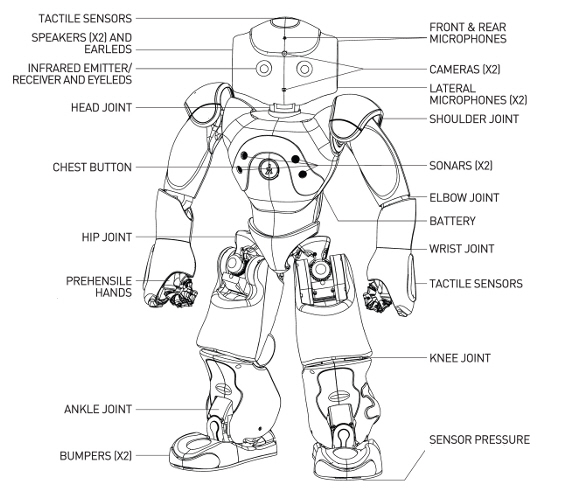
\includegraphics[scale=0.9]{Bilder/nao_overview.jpg}			
	\caption{Übersicht Nao V3.2}						
	\label{f:nao_ov}						
\end{figure}
\noindent
\textbf{Gelenke}
\\
Nao besitzt  im Kopf, den beiden Armen, dem Becken und den beiden Beinen jeweils mehrere Gelenke (\textit{Joint}, siehe Bild \ref{f:nao_ov}). Damit ist eine umfangreiche Bewegung in alle Richtungen der drei Achsen möglich. Der Kopf lässt sich in Z-Richtung drehen und in Y-Richtung neigen, damit Nao auch räumlich sehen bzw. Objekte verfolgen kann.
Die Arme besitzen die gleichen Gelenke wie in einem menschlichen Körper. Dazu gehören Schulter-, Ellenbogen- und Hangelenk. Das Schultergelenk dient dazu, den Arm zu heben/senken und ihn zu öffnen bzw. zu schließen. Das Drehen und Öffnen/Schließen des Unterarms geschieht durch das Ellenbogengelenk in Kombination mit dem Hangelenk. Die Finger der Hand können nur als Ganzes geöffnet bzw. geschlossen werden.
Das Beckengelenk wird dazu benutzt, den Torso von Nao nach vorne oder hinten zu neigen.
Die Beine bestehen aus drei Gelenken: Einem Hüft-, einem Knie- und einem Fußgelenk. Die Bewegungsfreiheit der Beine ähnelt dem des menschlichen Beins, wobei keines der Gelenke in Z-Richtung gedreht werden kann.

Die Bestimmung der Gelenkpositionen erfolgt über einen magnetischen Drehwinkelgeber	mit einer Auflösung von 12 Bit. Das macht beispielsweise bei einem Wert von 4096 pro Umdrehung eine Präzision von 0.1 Grad.
\\
\\
\textbf{Gelenkraum Nao}
\\
Da primär die Arme durch Nao nachgeahmt werden sollen, wird hier kurz auf den Gelenkraum dieser eingegangen. Jedes einzelne Gelenk der beiden Arme besitzt einen Winkelbereich in dem diese bewegt werden können. Tabellen \ref{tab:Lgelenkraum} und \ref{tab:Rgelenkraum} zeigen den Gelenkraum für den linken bzw. den rechten Arm.

\begin{table}[H]
    \begin{tabular}{|l|l|l|}
    \hline
    \textbf{Gelenk}         & \textbf{Bereich (Grad) } & \textbf{Bereich (Radian)}   \\
    \hline
    LShoulderPitch & -119.5 to 119.5 & -2.0857 to 2.0857  \\
    LShoulderRoll  & -18 to 76       & -0.3142 to 1.3265  \\
    LElbowYaw      & -119.5 to 119.5 & -2.0857 to 2.0857  \\
    LElbowRoll     & -88.5 to -2     & -1.5446 to -0.0349 \\
    LWristYaw      & -104.5 to 104.5 & -1.8238 to 1.8238  \\ \hline
    \end{tabular}
    \caption {Gelenkraum linker Arm}
    \label{tab:Lgelenkraum}
\end{table}
\begin{table}[H]
    \begin{tabular}{|l|l|l|}
    \hline
    \textbf{Gelenk}         & \textbf{Bereich (Grad) } & \textbf{Bereich (Radian)}   \\
    \hline
    RShoulderPitch & -119.5 to 119.5 & -2.0857 to 2.0857 \\
    RShoulderRoll  & -76 to 18       & -1.3265 to 0.3142 \\
    RElbowYaw      & -119.5 to 119.5 & -2.0857 to 2.0857 \\
    RElbowRoll     & 2 to 88.5       & 0.0349 to 1.5446  \\
    RWristYaw      & -104.5 to 104.5 & -1.8238 to 1.8238 \\ \hline
    \end{tabular}
    \caption {Gelenkraum rechter Arm}
    \label{tab:Rgelenkraum}
\end{table}
Bilder der einzelnen Gelenke und Winkelbereiche sind im Anhang zu finden.
\noindent
\textbf{Aktoren}
\\
In Nao sind vier verschiedene Typen von Motoren verbaut. Diese unterscheiden sich im wesentlichen in ihrer maximalen Anzahl an Drehungen pro Minute, dem Drehmoment und der Drehzahlrückstellung. Dies ist wichtig, da nicht jedes Gelenk und der zugehörige Aktor mit der gleichen Masse belastet wird.
\\
\\
\textbf{Elektronik \& Sensoren}
\\
Das Herz von Nao ist dessen Motherboard mit einer x86 AMD CPU mit 500MHz. Der Arbeitsspeicher mit 256MB RAM und die 2GB Flash-Speicher befinden sich zusammen mit dem Prozessor im Kopf.  Die Batterie mit rund 30Wh hält für die aktive Nutzung (viele Bewegungen und Sensoraktivitäten) ca. 60min und die normale Nutzung ca. 90min. 

Links und Rechts am Kopf befinden sich jeweils ein Lautsprecher und ein Mikrofon. Zusätliche Mikrofone sind am Kopf auch noch vorne und hinten angebracht. Damit ist es Nao möglich, ein Geräusch zu lokalisiern und gegebenenfalls dahin zu folgen. Um gleichzeitig die Ferne und die Nähe visuell zu verarbeiten wurde über und unter den Augen jeweils eine VGA - Kamera mit einer Auflösung von 640x480 Pixeln installiert. Die Augen selbst dienen zur Erkennung von Infrarotlicht, wobei auch hier in jedem Auge jeweils ein Sensor verbaut ist.

Auf der Brust von Nao befinden sich Ultraschallsensoren zur Distanzermittlung (je 2 Emitter und Empfänger). Diese haben eine Auflösung von 1cm und eine Erkennungsweite von 0.25m bis 2.55m. Unter 0.25m erkennt Nao nur noch, dass ein Objekt im Weg ist, aber nicht wie weit es entfernt ist.

Sensoren zur Kontakterkennung befinden sich auf dem Kopf, dem Brustbutton, auf und neben den Händen, sowie vorne an den Füßen. Unter den Füßen befinden sich zudem noch piezoresistive Drucksensoren mit einem Arbeitsbereich von 0 bis 25 Newton. Damit lässt sich unter anderem erkennen, ob Nao nur auf einem Bein oder auf unebenen Untergrund steht.


\section{Nao Software}
Um Nao auf einfache Weise zu programmieren, simulieren oder ihm neue Funktionen beizubringen, gibt es im wesentlichen zwei Programme. Diese werden im Folgenden jeweils kurz vorgestellt:
\\
\\
\noindent
\textbf{Choregraphe} 
\\
Choregraphe ist eine multi-plattform Desktopanwendung. Mit ihrer Hilfe ist es möglich:
\begin{itemize}
\item Neue Animationen und Verhalten zu erstellen,
\item diese entweder auf einem simulierten  oder direkt auf einem realen Roboter zu testen und
\item den Roboter dabei zu überwachen und zu steuern.
\end{itemize}
Dabei steht die Einfachheit der Anwendung im Vordergrund und so ist es auch möglich, sehr komplexes Verhalten (z.B. Interaktion mit Menschen, Tanzen oder E-Mails verschicken) zu implementieren ohne eine einzige Zeile Quellcode selbst zu schreiben. Zusätzlich ist die Möglichkeit gegeben, vorhandenen Code mit eigenem Python-Code zu erweitern.

\begin{figure}[H]						
	\centering							
	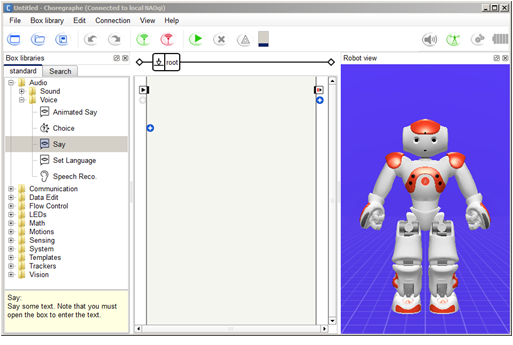
\includegraphics[scale=1.0]{Bilder/choregraphe.png}			
	\caption{Überblick Choregraphe}						
	\label{f:nao_choregraphe}						
\end{figure}
\noindent
Abbildung \ref{f:nao_choregraphe} zeigt einen Überblick über alle Subfenster und Panels innerhalb Choregraphe. Wie zu sehen, ist Choregraphe zentral in drei Bereiche unterteilt: Links, Mitte und Rechts.
Auf der linken Seite ist die sogenannte Box-Bibliothek zu finden. Dort sind alle von Haus aus gespeicherten Bewegungen und Verhalten abrufbar. Diese können per Drag \& Drop in die Mitte gezogen werden. Die Mitte stellt ein Fluss-Diagramm der einzelnen Boxen dar. So ist es möglich \textit{grafisch} zu programmieren (Verknüpfen der Boxen). Auf der rechten Seite ist das Abbild eines Nao-Roboters zu sehen. Dies zeigt, je nach dem, einen simulierten Roboter oder die Spiegelung eines realen Naos. 
Durch diese grafisch einfache Programmierung können auch unerfahrene Anwender mit Nao arbeiten. So ist er nicht nur für die Forschung oder für Entwickler gedacht, sondern auch für den Unterricht an Schulen.

Die Programmierung des Roboters geschieht durch Verbinden von einzelnen Boxen. Es ist auch möglich ein Programm mit verschiedenen Wegen zu entwerfen oder Konditionalstrukturen (\textit{if-else-elseif}) einzubauen. Abbildung \ref{f:nao_choregrapheProg} zeigt ein Programm, in welchem der Roboter zu einer gewissen Position laufen soll. Währenddessen überprüft er mittels Ultraschallsensor, ob ein Hindernis im Weg ist. Bei positivem Ergebnis soll sich der Roboter hinsetzen.

\begin{figure}[H]						
	\centering							
	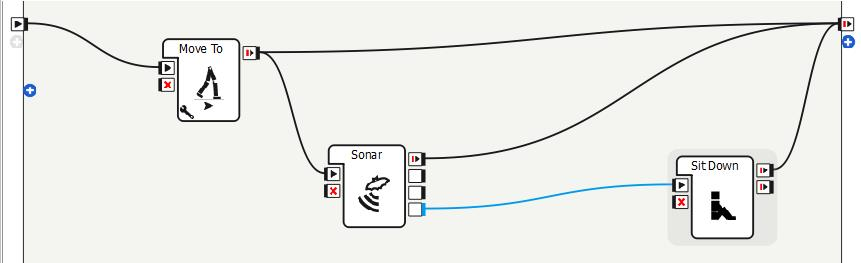
\includegraphics[scale=.6]{Bilder/choregraphe_prog.jpg}			
	\caption{Choregraphe Programmierung}						
	\label{f:nao_choregrapheProg}						
\end{figure}

Neue Bewegungen oder Verhalten können entweder durch eigenen Python-Code oder durch Vormachen integriert werden. Dazu kann über eine \textit{Timeline} aufgenommen werden, zu welchem Zeitpunkt der Bewegung sich die einzelnen Gelenke/Körperteile befinden sollen. Anschließend kann diese aufgenommene Timeline als Verhalten in einer Box gespeichert werden.
\\
\\
Die Möglichkeit neue Programme erst an einer Simulation zu testen, spart erstens Akkulaufzeit eines realen Nao und zweitens schützt es diesen vor \textit{schlechten} Programmen, bei denen er Schaden nehmen könnte. Ein weiterer Vorteil ist, dass zu jeder Box der Quellcode in Python sichtbar ist und sich dadurch Arbeit erspart werden kann.
\\
\\
Choregraphe wurde in dieser Arbeit hauptsächlich dazu genutzt, sich in die Marterie Nao einzuarbeiten, seine Funktionsweise zu verstehen und zu erlernen wie er programmiert wird.
\\
\\
\textbf{Webots for Nao}
\\
Webots für Nao erlaubt es, einen simulierten Roboter in einer virtuellen Welt zu bewegen. Die Software bietet eine sichere Umgebung, um neue Verhalten zu testen, bevor sie in die reale Welt übertragen werden. Webots for Nao ist eine spezifische Auskopplung von Webots 7, einer professionellen Software zum Simulieren diverser Roboter, beispielsweise KUKA-Robotern oder Lego Mindstorms. Mit Webots for Nao können jedoch keine anderen Roboter genutzt oder neue erstellt werden.

\begin{figure}[H]						
	\centering							
	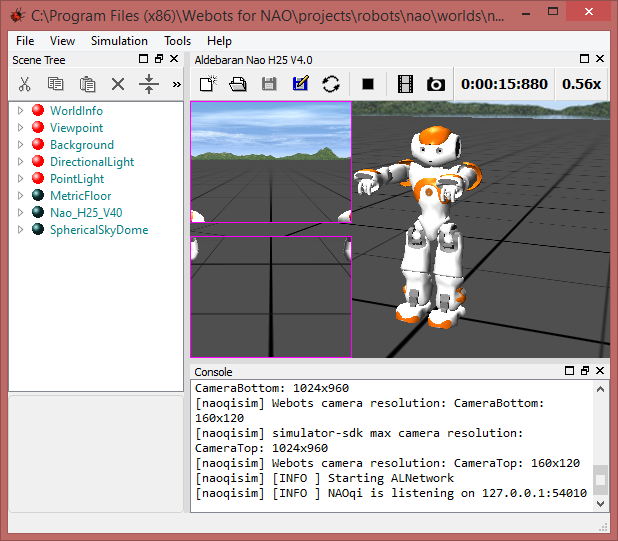
\includegraphics[scale=1.0]{Bilder/webots.png}			
	\caption{Überblick Webots}						
	\label{f:nao_webots}						
\end{figure}
\noindent
Bild \myref{f:nao_webots} zeigt einen simulierten Nao in einer virtuellen Welt. Auf der linken Seite befinden sich Reiter, die ausgeklappt werden können. Dort können Objekte in die Welt gelegt werden. Auf der rechten Seite ist Nao von vorne und jeweils ein Ausschnitt der beiden Kameras an seinem Kopf zu sehen. Unterhalb davon ist eine Konsole, die verschiedene Angaben ausgibt, z.B. die IP-Adresse und der Port, unter dem der simulierte Nao angesprochen werden kann.

Der Unterschied zu der Simulation in Choregraphe liegt darin, dass in Webots auch Elemente wie Tische, Stühle oder andere Hindernisse in die Welt gelegt werden können. So kann beispielsweise getestet werden, ob Nao Hindernissen ausweicht, wenn er auf sie zu läuft.
\\
\\
Webots wurde im Allgemeinen dafür genutzt zu Testen, ob die Übertragung der Armwinkel korrekt ist und ob diese der Bewegung durch den Menschen entsprechen. Würden die Tests an einem realen Nao durchgeführt werden, währen seine Aktoren sehr schnell warm und könnten eventuell Schaden davon nehmen.






\section{NAOqi Framework}

NAOqi ist der Name der Software die tatsächlich auf dem Roboter läuft und ihn kontrolliert. Das NAOqi Framework ist das Gerüst um Nao zu programmieren. Es spricht auf die gewöhnlichen Anforderungen in der Robotertechnik an: Parallelität (von Threads), Ressourcen, Synchronisation und Events. Das bedeutet, es kann mit allen gängigen Techniken der Software - Entwicklung bedient werden. 

Dieses Framework erlaubt homogene Kommunikation zwischen verschiedenen Modulen (Bewegung, Autio, Video), homogene Programmierung und homogenes Teilen von Informationen über die verschiedenen Module hinweg.
\\
\\
\noindent
\myref{f:naoqi_ov} zeigt die einzelnen Komponenten des NAOqi Frameworks:
\begin{itemize}
\item Cross - Plattform
\item Cross - Language
\item NAOqi - Prozess
\item Module
\end{itemize}

\begin{figure}[H]						
	\centering							
	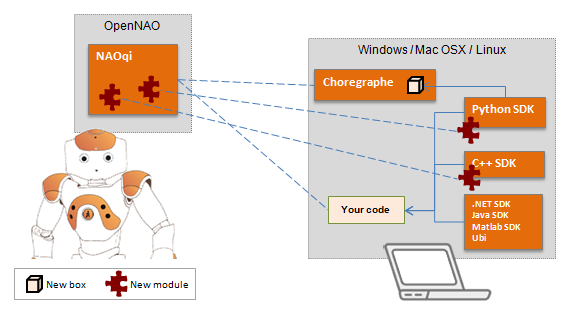
\includegraphics[scale=0.8]{Bilder/naoqi_ov.PNG}
	\caption{NAOqi Übersicht}						
	\label{f:naoqi_ov}						
\end{figure}


\subsection{Cross - Plattform/Language}

\textbf{Cross - Plattform}
\\
Cross - Plattform bedeutet Plattformunabhängigkeit gegenüber dem Betriebssystem auf dem Programmiert werden soll. Sowohl auf Linux, Windows und auf Mac kann Code für Nao programmiert werden. Allerdings kann auf Windows und Mac nur Code auf dem Computer selbst kompiliert werden, während auf Linux der Code auch auf dem Roboter selbst programmiert werden kann.
\\
\\
\textbf{Cross - Language}
\\	
Cross - Language ist nach \cite{ws:naodocu} die Eigenschaft, dass Software in C++ und in Python entwickelt werden kann. In allen Fällen, in denen die Methoden exakt gleich sind kann die \ac{API} (dt: Programmierschnittstelle), gleichgültig von welcher der unterstützten Programmiersprachen, aufgerufen werden. Die \ac{API} ist in acht Programmiersprachen verfügbar: C++, Python, .NET (C\#, Visual Basic, F\#), Java, Matlab und Urbi.

Neue NAOqi Module können nur in C++ oder Python entwickelt werden, jedoch kann die Client - API mit allen Programmiersprachen angesprochen werden. Ebenso sind nur C++ und Python auf dem Roboter unterstützt, die anderen Sprachen werden nur über \textit{Remote - Access} unterstützt. (siehe unten \textit{Proxy})
\\
\subsection{NAOqi - Prozess}
Der NAOqi - Prozess der auf dem Roboter läuft ist ein \textit{Broker} (siehe unten). Beim Start des Prozesses wird eine Konfigurationsdatei \textsf{autoload.ini} geladen, die definiert, welche Bibliotheken geladen werden sollen. Jede Bibliothek beinhaltet ein oder mehrere Module, die der Broker nutzt um deren Methoden öffentlich anzuzeigen. (siehe \ref{f:naoqi_broker1})

\begin{figure}[H]						
	\centering							
	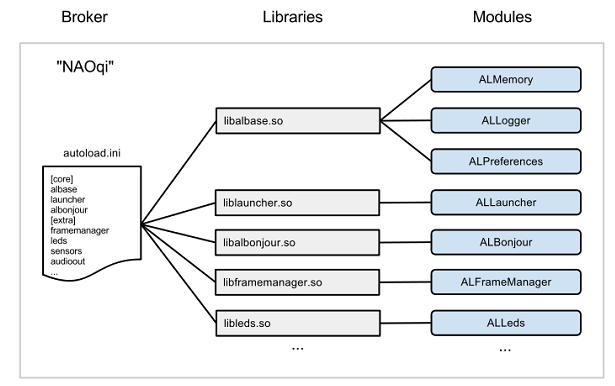
\includegraphics[scale=0.8]{Bilder/naoqi_process1.PNG}
	\caption{NAOqi Broker}						
	\label{f:naoqi_broker1}						
\end{figure}

Der Broker 	stellt einen Lookup - Service zu Verfügung, so dass jedes Modul im Baum oder verteilt im Netzwerk jede Methode finden kann, die öffentlich angezeigt wurde.

Das Laden der Module zum Start erzeugt einen Baum von Methoden, die an Module geknüpft und diese wiederum an einen Broker geknüpft sind. (siehe \ref{f:naoqi_broker2})

\begin{figure}[H]						
	\centering							
	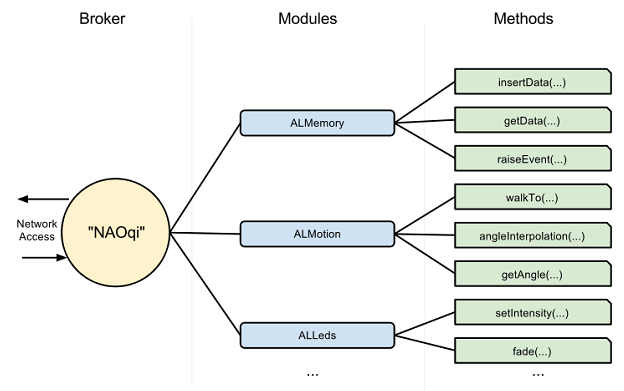
\includegraphics[scale=0.8]{Bilder/naoqi_process2.PNG}
	\caption{NAOqi Method-Tree}						
	\label{f:naoqi_broker2}						
\end{figure}
\noindent
\textbf{Broker}
\\
Der Broker ist ein Objekt, der zwei generelle Rollen einnimmt. Erstens ist das ein Verzeichnis - Dienst, mit dessen Hilfe Module und Methoden gefunden werden können und zweitens ein Netzwerk - Anschluss, der es möglich macht Methoden verknüpfter Module auch außerhalb des Prozesses aufzurufen.

Die Meiste Zeit muss sich keine Gedanken um die Broker gemacht werden, da diese ihre Arbeit selbstständig und transparent machen. Geschriebener Code kann gleich sein, ob für Aufrufe an "`remote Module"' (dt.: entfernt; anderer Prozess oder anderes System) oder "`lokale Module"' (gleicher Prozess).
\\
\\
\textbf{Proxy}
\\
Ein Proxy ist ein Stellvertreter - Objekt das sich genau so verhält, wie das Modul das es repräsentiert. Wenn ein Proxy - Objekt des ALMotion Moduls instanziiert wird, erhält das Proxy - Objekt auch alle Methoden des ALMotion Moduls.

Um ein Proxy eines Moduls zu instanziieren gibt es zwei Möglichkeiten: 
\begin{itemize}
\item Nur den Namen des Moduls benutzen. In diesem Fall muss der auszuführende Code und das Modul das verbunden werden soll im selben Broker liegen. Dies ist ein "`lokaler"' Aufruf
\item Zusätzlich zum Namen des Moduls auch die IP und den Port des Broker benutzen. In diesem Fall muss das Modul im zugehörigen Broker liegen. Dies ist ein "`remote"' Aufruf.
\end{itemize}
Der genaue Unterschied zwischen "`remote"' und "`lokalen"' Modulen wird im folgenden erklärt.
\\
\subsection{Module}
Typischerweise ist ein Modul eine Klasse innerhalb einer Bibliothek und wird automatisch instanziiert wenn diese  durch \textsf{autoload.ini} geladen wird. Neue Methoden können an Klassen gebunden werden, die von \textsf{ALModule} erben. Dadurch werden die Methoden mit ihrem Namen und ihrer Signatur dem Broker öffentlich gemacht, so dass diese anderen verfügbar wird.

Ein Modul kann, wie oben bereits erwähnt, entweder "`remote"' oder "`lokal"' sein. 

\textbf{Lokale Module } sind zwei (oder mehr) Module, die im selben Prozess gestartet wurden. Sie kommunizieren miteinander lediglich über \textbf{einen} Broker. Durch den gemeinsamen Prozess können sie sich  Variablen teilen und einander Methoden ohne Serialisierung oder Netzwerkverbindung aufrufen. Dies erlaubt die schnellste Kommunikation untereinander. Lokale Module werden als Bibliothek kompiliert und können ausschließlich auf dem Roboter ausgeführt werden. Sie sind sehr schnell und effizient im Umgang mit dem Arbeitsspeicher.

\textbf{Remote Module} kommunizieren über das Netzwerk miteinander. Jedes remote Module benötigt einen Broker um mit anderen Modulen zu sprechen. Der Broker nutzt dabei das Netzwerkprotokoll SOAP\footnote{Simple Object Access Protocol, dient u.a. dazu \textit{Remoe Procedure Calls} durchzuführen} um die Kommunikation bereitzustellen. Schnelles Ansprechen von Modulen ist über ein remote Modul nicht möglich, beispielsweise bei direkter Adressierung des Arbeitsspeichers. Remote Module werden als ausführbare Dateien kompiliert und können außerhalb des Roboters aufgerufen werden. Remote Module sind einfacher zu benutzen und können dadurch von außen einfacher debuggt werden. Allerdings sind sie langsamer und weit weniger effizient wie lokale Module. 
\\
Die Kommunikation zwischen remote Modulen kann über zwei Wege erfolgen. Erstens \textbf{Broker to Broker} und zweitens \textbf{Proxy to Broker}.
 
Der Unterschied liegt darin, dass Broker to Broker eine wechselseitige, Proxy to Broker nur eine einseitige Kommunikation eröffnet. Bei zwei Modulen B und C kann bei Broker to Broker B Methoden von C und C Methoden von B aufrufen. Bei Proxy to Broker ist dies nur in die Richtung von B nach C möglich, nicht umgekehrt. Folgendes Listing zeigt die Implementierung beider Kommunikationsarten.

\lstinputlisting
    [caption={Kommunikationsarten Module}
       \label{test},
       captionpos=b]	
 {Listings/module_comm.cs}
\noindent	
\textbf{Blocking und non - Blocking Aufrufe}
\\



\subsection{.NET SDK}
vorstellung c\# SDK, HelloWorld
\chapter{Nao}\label{c:nao}
Nao ist ein humanoider Roboter des französischen Herstellers \textit{Aldebaran Robotic}. Die erste Version des Roboters wurde 2006 vorgestellt und unter anderem mit einem Investment durch Intel weiterentwickelt. Es gibt den Roboter in verschiedenen Ausführungen mit verschieden verbauten Sensoren und kostet ungefähr 10.000 Euro. \cite{ws:wikinao}

Im folgenden Kapitel wird der Aufbau und die Funktionen der Hardware, sowie die zugehörige Software zur Bedienung und Programmierung des Nao vorgestellt.

\section{Nao Hardware}
\label{nao:hardware}
Der in dieser Arbeit verwendete Nao ist vom Typ \textit{NAO V3+, V3.2}. Dieser Typ ist 573.2 mm hoch, 290 mm tief und 273.3 mm breit. In Abbildung \myref{f:nao_ov} sind alle Sensoren und Aktoren aufgeführt.
\\
\begin{figure}[H]						
	\centering							
	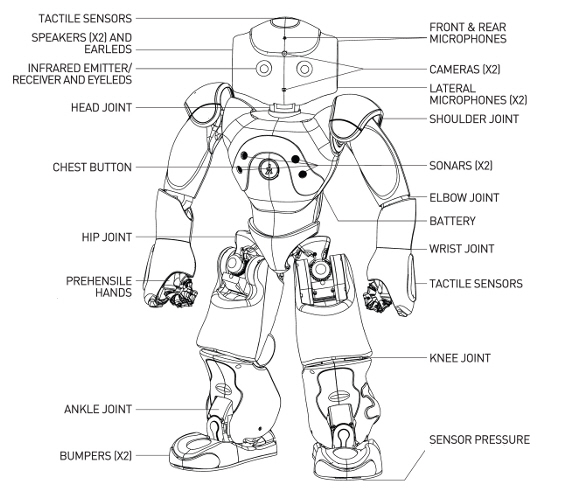
\includegraphics[scale=0.9]{Bilder/nao_overview.jpg}			
	\caption{Übersicht Nao V3.2}						
	\label{f:nao_ov}						
\end{figure}
\noindent
\textbf{Gelenke}
\\
Nao besitzt  im Kopf, den beiden Armen, dem Becken und den beiden Beinen jeweils mehrere Gelenke (\textit{Joint}, siehe Bild \ref{f:nao_ov}). Damit ist eine umfangreiche Bewegung in alle Richtungen der drei Achsen möglich. Der Kopf lässt sich in Z-Richtung drehen und in Y-Richtung neigen, damit Nao auch räumlich sehen bzw. Objekte verfolgen kann.
Die Arme besitzen die gleichen Gelenke wie in einem menschlichen Körper. Dazu gehören Schulter-, Ellenbogen- und Hangelenk. Das Schultergelenk dient dazu, den Arm zu heben/senken und ihn zu öffnen bzw. zu schließen. Das Drehen und Öffnen/Schließen des Unterarms geschieht durch das Ellenbogengelenk in Kombination mit dem Hangelenk. Die Finger der Hand können nur als Ganzes geöffnet bzw. geschlossen werden.
Das Beckengelenk wird dazu benutzt, den Torso von Nao nach vorne oder hinten zu neigen.
Die Beine bestehen aus drei Gelenken: Einem Hüft-, einem Knie- und einem Fußgelenk. Die Bewegungsfreiheit der Beine ähnelt dem des menschlichen Beins, wobei keines der Gelenke in Z-Richtung gedreht werden kann.

Die Bestimmung der Gelenkpositionen erfolgt über einen magnetischen Drehwinkelgeber	mit einer Auflösung von 12 Bit. Das macht beispielsweise bei einem Wert von 4096 pro Umdrehung eine Präzision von 0.1 Grad.
\\
\\
\textbf{Gelenkraum Nao}
\\
Da primär die Arme durch Nao nachgeahmt werden sollen, wird hier kurz auf den Gelenkraum dieser eingegangen. Jedes einzelne Gelenk der beiden Arme besitzt einen Winkelbereich in dem diese bewegt werden können. Tabellen \ref{tab:Lgelenkraum} und \ref{tab:Rgelenkraum} zeigen den Gelenkraum für den linken bzw. den rechten Arm.

\begin{table}[H]
    \begin{tabular}{|l|l|l|}
    \hline
    \textbf{Gelenk}         & \textbf{Bereich (Grad) } & \textbf{Bereich (Radian)}   \\
    \hline
    LShoulderPitch & -119.5 to 119.5 & -2.0857 to 2.0857  \\
    LShoulderRoll  & -18 to 76       & -0.3142 to 1.3265  \\
    LElbowYaw      & -119.5 to 119.5 & -2.0857 to 2.0857  \\
    LElbowRoll     & -88.5 to -2     & -1.5446 to -0.0349 \\
    LWristYaw      & -104.5 to 104.5 & -1.8238 to 1.8238  \\ \hline
    \end{tabular}
    \caption {Gelenkraum linker Arm}
    \label{tab:Lgelenkraum}
\end{table}
\begin{table}[H]
    \begin{tabular}{|l|l|l|}
    \hline
    \textbf{Gelenk}         & \textbf{Bereich (Grad) } & \textbf{Bereich (Radian)}   \\
    \hline
    RShoulderPitch & -119.5 to 119.5 & -2.0857 to 2.0857 \\
    RShoulderRoll  & -76 to 18       & -1.3265 to 0.3142 \\
    RElbowYaw      & -119.5 to 119.5 & -2.0857 to 2.0857 \\
    RElbowRoll     & 2 to 88.5       & 0.0349 to 1.5446  \\
    RWristYaw      & -104.5 to 104.5 & -1.8238 to 1.8238 \\ \hline
    \end{tabular}
    \caption {Gelenkraum rechter Arm}
    \label{tab:Rgelenkraum}
\end{table}
Bilder der einzelnen Gelenke und Winkelbereiche sind im Anhang zu finden.
\noindent
\textbf{Aktoren}
\\
In Nao sind vier verschiedene Typen von Motoren verbaut. Diese unterscheiden sich im wesentlichen in ihrer maximalen Anzahl an Drehungen pro Minute, dem Drehmoment und der Drehzahlrückstellung. Dies ist wichtig, da nicht jedes Gelenk und der zugehörige Aktor mit der gleichen Masse belastet wird.
\\
\\
\textbf{Elektronik \& Sensoren}
\\
Das Herz von Nao ist dessen Motherboard mit einer x86 AMD CPU mit 500MHz. Der Arbeitsspeicher mit 256MB RAM und die 2GB Flash-Speicher befinden sich zusammen mit dem Prozessor im Kopf.  Die Batterie mit rund 30Wh hält für die aktive Nutzung (viele Bewegungen und Sensoraktivitäten) ca. 60min und die normale Nutzung ca. 90min. 

Links und Rechts am Kopf befinden sich jeweils ein Lautsprecher und ein Mikrofon. Zusätliche Mikrofone sind am Kopf auch noch vorne und hinten angebracht. Damit ist es Nao möglich, ein Geräusch zu lokalisiern und gegebenenfalls dahin zu folgen. Um gleichzeitig die Ferne und die Nähe visuell zu verarbeiten wurde über und unter den Augen jeweils eine VGA - Kamera mit einer Auflösung von 640x480 Pixeln installiert. Die Augen selbst dienen zur Erkennung von Infrarotlicht, wobei auch hier in jedem Auge jeweils ein Sensor verbaut ist.

Auf der Brust von Nao befinden sich Ultraschallsensoren zur Distanzermittlung (je 2 Emitter und Empfänger). Diese haben eine Auflösung von 1cm und eine Erkennungsweite von 0.25m bis 2.55m. Unter 0.25m erkennt Nao nur noch, dass ein Objekt im Weg ist, aber nicht wie weit es entfernt ist.

Sensoren zur Kontakterkennung befinden sich auf dem Kopf, dem Brustbutton, auf und neben den Händen, sowie vorne an den Füßen. Unter den Füßen befinden sich zudem noch piezoresistive Drucksensoren mit einem Arbeitsbereich von 0 bis 25 Newton. Damit lässt sich unter anderem erkennen, ob Nao nur auf einem Bein oder auf unebenen Untergrund steht.


\section{Nao Software}
Um Nao auf einfache Weise zu programmieren, simulieren oder ihm neue Funktionen beizubringen, gibt es im wesentlichen zwei Programme. Diese werden im Folgenden jeweils kurz vorgestellt:
\\
\\
\noindent
\textbf{Choregraphe} 
\\
Choregraphe ist eine multi-plattform Desktopanwendung. Mit ihrer Hilfe ist es möglich:
\begin{itemize}
\item Neue Animationen und Verhalten zu erstellen,
\item diese entweder auf einem simulierten  oder direkt auf einem realen Roboter zu testen und
\item den Roboter dabei zu überwachen und zu steuern.
\end{itemize}
Dabei steht die Einfachheit der Anwendung im Vordergrund und so ist es auch möglich, sehr komplexes Verhalten (z.B. Interaktion mit Menschen, Tanzen oder E-Mails verschicken) zu implementieren ohne eine einzige Zeile Quellcode selbst zu schreiben. Zusätzlich ist die Möglichkeit gegeben, vorhandenen Code mit eigenem Python-Code zu erweitern.

\begin{figure}[H]						
	\centering							
	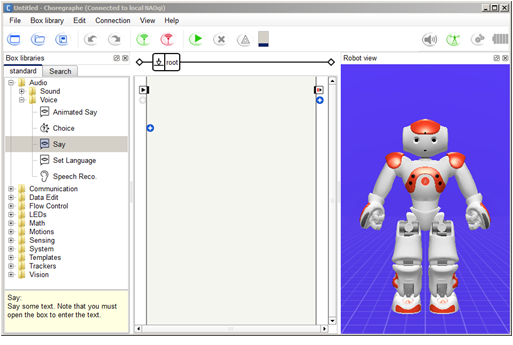
\includegraphics[scale=1.0]{Bilder/choregraphe.png}			
	\caption{Überblick Choregraphe}						
	\label{f:nao_choregraphe}						
\end{figure}
\noindent
Abbildung \ref{f:nao_choregraphe} zeigt einen Überblick über alle Subfenster und Panels innerhalb Choregraphe. Wie zu sehen, ist Choregraphe zentral in drei Bereiche unterteilt: Links, Mitte und Rechts.
Auf der linken Seite ist die sogenannte Box-Bibliothek zu finden. Dort sind alle von Haus aus gespeicherten Bewegungen und Verhalten abrufbar. Diese können per Drag \& Drop in die Mitte gezogen werden. Die Mitte stellt ein Fluss-Diagramm der einzelnen Boxen dar. So ist es möglich \textit{grafisch} zu programmieren (Verknüpfen der Boxen). Auf der rechten Seite ist das Abbild eines Nao-Roboters zu sehen. Dies zeigt, je nach dem, einen simulierten Roboter oder die Spiegelung eines realen Naos. 
Durch diese grafisch einfache Programmierung können auch unerfahrene Anwender mit Nao arbeiten. So ist er nicht nur für die Forschung oder für Entwickler gedacht, sondern auch für den Unterricht an Schulen.

Die Programmierung des Roboters geschieht durch Verbinden von einzelnen Boxen. Es ist auch möglich ein Programm mit verschiedenen Wegen zu entwerfen oder Konditionalstrukturen (\textit{if-else-elseif}) einzubauen. Abbildung \ref{f:nao_choregrapheProg} zeigt ein Programm, in welchem der Roboter zu einer gewissen Position laufen soll. Währenddessen überprüft er mittels Ultraschallsensor, ob ein Hindernis im Weg ist. Bei positivem Ergebnis soll sich der Roboter hinsetzen.

\begin{figure}[H]						
	\centering							
	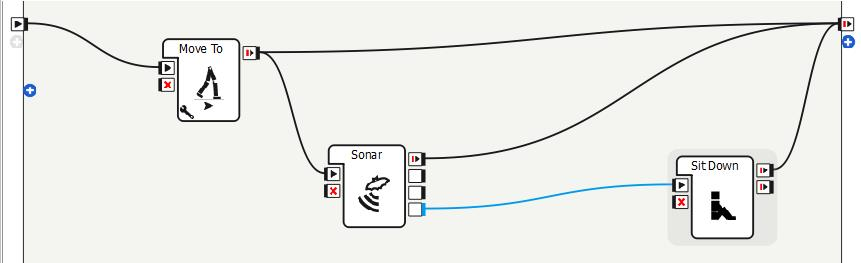
\includegraphics[scale=.6]{Bilder/choregraphe_prog.jpg}			
	\caption{Choregraphe Programmierung}						
	\label{f:nao_choregrapheProg}						
\end{figure}

Neue Bewegungen oder Verhalten können entweder durch eigenen Python-Code oder durch Vormachen integriert werden. Dazu kann über eine \textit{Timeline} aufgenommen werden, zu welchem Zeitpunkt der Bewegung sich die einzelnen Gelenke/Körperteile befinden sollen. Anschließend kann diese aufgenommene Timeline als Verhalten in einer Box gespeichert werden.
\\
\\
Die Möglichkeit neue Programme erst an einer Simulation zu testen, spart erstens Akkulaufzeit eines realen Nao und zweitens schützt es diesen vor \textit{schlechten} Programmen, bei denen er Schaden nehmen könnte. Ein weiterer Vorteil ist, dass zu jeder Box der Quellcode in Python sichtbar ist und sich dadurch Arbeit erspart werden kann.
\\
\\
Choregraphe wurde in dieser Arbeit hauptsächlich dazu genutzt, sich in die Marterie Nao einzuarbeiten, seine Funktionsweise zu verstehen und zu erlernen wie er programmiert wird.
\\
\\
\textbf{Webots for Nao}
\\
Webots für Nao erlaubt es, einen simulierten Roboter in einer virtuellen Welt zu bewegen. Die Software bietet eine sichere Umgebung, um neue Verhalten zu testen, bevor sie in die reale Welt übertragen werden. Webots for Nao ist eine spezifische Auskopplung von Webots 7, einer professionellen Software zum Simulieren diverser Roboter, beispielsweise KUKA-Robotern oder Lego Mindstorms. Mit Webots for Nao können jedoch keine anderen Roboter genutzt oder neue erstellt werden.

\begin{figure}[H]						
	\centering							
	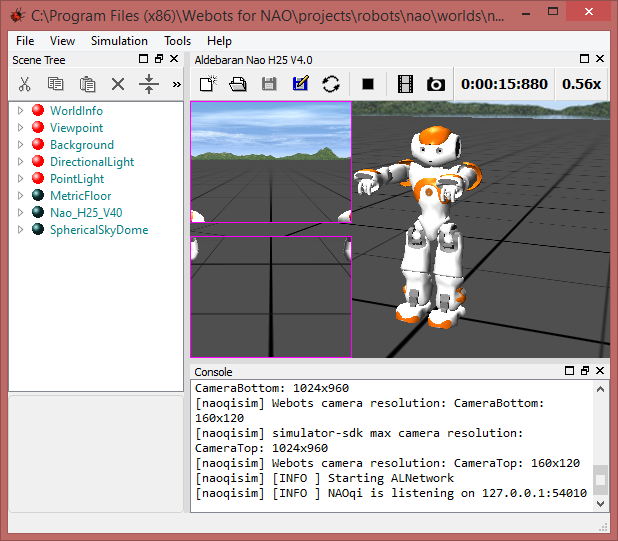
\includegraphics[scale=1.0]{Bilder/webots.png}			
	\caption{Überblick Webots}						
	\label{f:nao_webots}						
\end{figure}
\noindent
Bild \myref{f:nao_webots} zeigt einen simulierten Nao in einer virtuellen Welt. Auf der linken Seite befinden sich Reiter, die ausgeklappt werden können. Dort können Objekte in die Welt gelegt werden. Auf der rechten Seite ist Nao von vorne und jeweils ein Ausschnitt der beiden Kameras an seinem Kopf zu sehen. Unterhalb davon ist eine Konsole, die verschiedene Angaben ausgibt, z.B. die IP-Adresse und der Port, unter dem der simulierte Nao angesprochen werden kann.

Der Unterschied zu der Simulation in Choregraphe liegt darin, dass in Webots auch Elemente wie Tische, Stühle oder andere Hindernisse in die Welt gelegt werden können. So kann beispielsweise getestet werden, ob Nao Hindernissen ausweicht, wenn er auf sie zu läuft.
\\
\\
Webots wurde im Allgemeinen dafür genutzt zu Testen, ob die Übertragung der Armwinkel korrekt ist und ob diese der Bewegung durch den Menschen entsprechen. Würden die Tests an einem realen Nao durchgeführt werden, währen seine Aktoren sehr schnell warm und könnten eventuell Schaden davon nehmen.






\section{NAOqi Framework}

NAOqi ist der Name der Software die tatsächlich auf dem Roboter läuft und ihn kontrolliert. Das NAOqi Framework ist das Gerüst um Nao zu programmieren. Es spricht auf die gewöhnlichen Anforderungen in der Robotertechnik an: Parallelität (von Threads), Ressourcen, Synchronisation und Events. Das bedeutet, es kann mit allen gängigen Techniken der Software - Entwicklung bedient werden. 

Dieses Framework erlaubt homogene Kommunikation zwischen verschiedenen Modulen (Bewegung, Autio, Video), homogene Programmierung und homogenes Teilen von Informationen über die verschiedenen Module hinweg.
\\
\\
\noindent
\myref{f:naoqi_ov} zeigt die einzelnen Komponenten des NAOqi Frameworks:
\begin{itemize}
\item Cross - Plattform
\item Cross - Language
\item NAOqi - Prozess
\item Module
\end{itemize}

\begin{figure}[H]						
	\centering							
	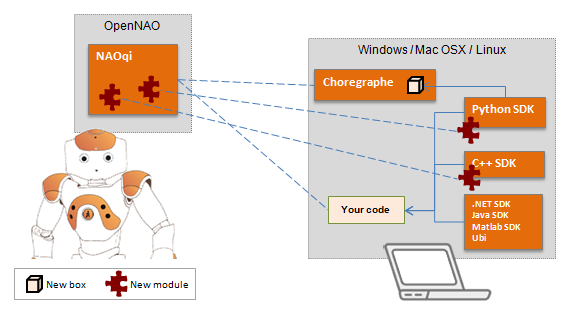
\includegraphics[scale=0.8]{Bilder/naoqi_ov.PNG}
	\caption{NAOqi Übersicht}						
	\label{f:naoqi_ov}						
\end{figure}


\subsection{Cross - Plattform/Language}

\textbf{Cross - Plattform}
\\
Cross - Plattform bedeutet Plattformunabhängigkeit gegenüber dem Betriebssystem auf dem Programmiert werden soll. Sowohl auf Linux, Windows und auf Mac kann Code für Nao programmiert werden. Allerdings kann auf Windows und Mac nur Code auf dem Computer selbst kompiliert werden, während auf Linux der Code auch auf dem Roboter selbst programmiert werden kann.
\\
\\
\textbf{Cross - Language}
\\	
Cross - Language ist nach \cite{ws:naodocu} die Eigenschaft, dass Software in C++ und in Python entwickelt werden kann. In allen Fällen, in denen die Methoden exakt gleich sind kann die \ac{API} (dt: Programmierschnittstelle), gleichgültig von welcher der unterstützten Programmiersprachen, aufgerufen werden. Die \ac{API} ist in acht Programmiersprachen verfügbar: C++, Python, .NET (C\#, Visual Basic, F\#), Java, Matlab und Urbi.

Neue NAOqi Module können nur in C++ oder Python entwickelt werden, jedoch kann die Client - API mit allen Programmiersprachen angesprochen werden. Ebenso sind nur C++ und Python auf dem Roboter unterstützt, die anderen Sprachen werden nur über \textit{Remote - Access} unterstützt. (siehe unten \textit{Proxy})
\\
\subsection{NAOqi - Prozess}
Der NAOqi - Prozess der auf dem Roboter läuft ist ein \textit{Broker} (siehe unten). Beim Start des Prozesses wird eine Konfigurationsdatei \textsf{autoload.ini} geladen, die definiert, welche Bibliotheken geladen werden sollen. Jede Bibliothek beinhaltet ein oder mehrere Module, die der Broker nutzt um deren Methoden öffentlich anzuzeigen. (siehe \ref{f:naoqi_broker1})

\begin{figure}[H]						
	\centering							
	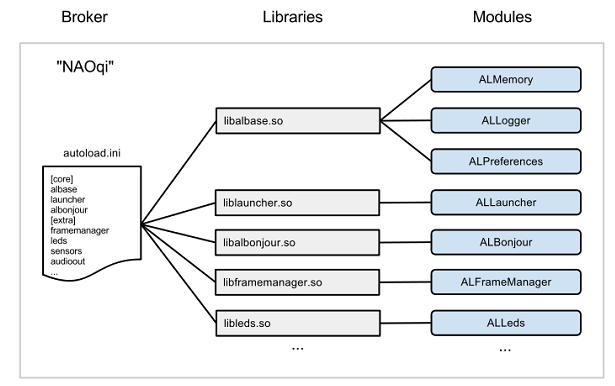
\includegraphics[scale=0.8]{Bilder/naoqi_process1.PNG}
	\caption{NAOqi Broker}						
	\label{f:naoqi_broker1}						
\end{figure}

Der Broker 	stellt einen Lookup - Service zu Verfügung, so dass jedes Modul im Baum oder verteilt im Netzwerk jede Methode finden kann, die öffentlich angezeigt wurde.

Das Laden der Module zum Start erzeugt einen Baum von Methoden, die an Module geknüpft und diese wiederum an einen Broker geknüpft sind. (siehe \ref{f:naoqi_broker2})

\begin{figure}[H]						
	\centering							
	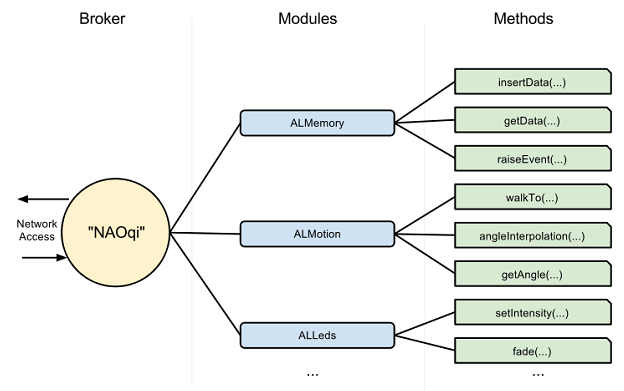
\includegraphics[scale=0.8]{Bilder/naoqi_process2.PNG}
	\caption{NAOqi Method-Tree}						
	\label{f:naoqi_broker2}						
\end{figure}
\noindent
\textbf{Broker}
\\
Der Broker ist ein Objekt, der zwei generelle Rollen einnimmt. Erstens ist das ein Verzeichnis - Dienst, mit dessen Hilfe Module und Methoden gefunden werden können und zweitens ein Netzwerk - Anschluss, der es möglich macht Methoden verknüpfter Module auch außerhalb des Prozesses aufzurufen.

Die Meiste Zeit muss sich keine Gedanken um die Broker gemacht werden, da diese ihre Arbeit selbstständig und transparent machen. Geschriebener Code kann gleich sein, ob für Aufrufe an "`remote Module"' (dt.: entfernt; anderer Prozess oder anderes System) oder "`lokale Module"' (gleicher Prozess).
\\
\\
\textbf{Proxy}
\\
Ein Proxy ist ein Stellvertreter - Objekt das sich genau so verhält, wie das Modul das es repräsentiert. Wenn ein Proxy - Objekt des ALMotion Moduls instanziiert wird, erhält das Proxy - Objekt auch alle Methoden des ALMotion Moduls.

Um ein Proxy eines Moduls zu instanziieren gibt es zwei Möglichkeiten: 
\begin{itemize}
\item Nur den Namen des Moduls benutzen. In diesem Fall muss der auszuführende Code und das Modul das verbunden werden soll im selben Broker liegen. Dies ist ein "`lokaler"' Aufruf
\item Zusätzlich zum Namen des Moduls auch die IP und den Port des Broker benutzen. In diesem Fall muss das Modul im zugehörigen Broker liegen. Dies ist ein "`remote"' Aufruf.
\end{itemize}
Der genaue Unterschied zwischen "`remote"' und "`lokalen"' Modulen wird im folgenden erklärt.
\\
\subsection{Module}
Typischerweise ist ein Modul eine Klasse innerhalb einer Bibliothek und wird automatisch instanziiert wenn diese  durch \textsf{autoload.ini} geladen wird. Neue Methoden können an Klassen gebunden werden, die von \textsf{ALModule} erben. Dadurch werden die Methoden mit ihrem Namen und ihrer Signatur dem Broker öffentlich gemacht, so dass diese anderen verfügbar wird.

Ein Modul kann, wie oben bereits erwähnt, entweder "`remote"' oder "`lokal"' sein. 

\textbf{Lokale Module } sind zwei (oder mehr) Module, die im selben Prozess gestartet wurden. Sie kommunizieren miteinander lediglich über \textbf{einen} Broker. Durch den gemeinsamen Prozess können sie sich  Variablen teilen und einander Methoden ohne Serialisierung oder Netzwerkverbindung aufrufen. Dies erlaubt die schnellste Kommunikation untereinander. Lokale Module werden als Bibliothek kompiliert und können ausschließlich auf dem Roboter ausgeführt werden. Sie sind sehr schnell und effizient im Umgang mit dem Arbeitsspeicher.

\textbf{Remote Module} kommunizieren über das Netzwerk miteinander. Jedes remote Module benötigt einen Broker um mit anderen Modulen zu sprechen. Der Broker nutzt dabei das Netzwerkprotokoll SOAP\footnote{Simple Object Access Protocol, dient u.a. dazu \textit{Remoe Procedure Calls} durchzuführen} um die Kommunikation bereitzustellen. Schnelles Ansprechen von Modulen ist über ein remote Modul nicht möglich, beispielsweise bei direkter Adressierung des Arbeitsspeichers. Remote Module werden als ausführbare Dateien kompiliert und können außerhalb des Roboters aufgerufen werden. Remote Module sind einfacher zu benutzen und können dadurch von außen einfacher debuggt werden. Allerdings sind sie langsamer und weit weniger effizient wie lokale Module. 
\\
Die Kommunikation zwischen remote Modulen kann über zwei Wege erfolgen. Erstens \textbf{Broker to Broker} und zweitens \textbf{Proxy to Broker}.
 
Der Unterschied liegt darin, dass Broker to Broker eine wechselseitige, Proxy to Broker nur eine einseitige Kommunikation eröffnet. Bei zwei Modulen B und C kann bei Broker to Broker B Methoden von C und C Methoden von B aufrufen. Bei Proxy to Broker ist dies nur in die Richtung von B nach C möglich, nicht umgekehrt. Folgendes Listing zeigt die Implementierung beider Kommunikationsarten.

\lstinputlisting
    [caption={Kommunikationsarten Module}
       \label{test},
       captionpos=b]	
 {Listings/module_comm.cs}
\noindent	
\textbf{Blocking und non - Blocking Aufrufe}
\\



\subsection{.NET SDK}
vorstellung c\# SDK, HelloWorld

\chapter{Realisierung}
In diesem Kapitel wird näher auf das Zusammenspiel von Sensorik (Kinect) und Aktorik (Nao) eingegangen. Zunächst wird die Idee der Softwarearchitektur vorgestellt. Im Anschluss daran, wird auf die entworfenen Algorithmen näher eingegangen.

\todo(Wahl Bibliothek, warum?...)
\todo{Laborbedingungen Steuerungen, Vor- und Nachteile der Bedienung}

%%
%
%	Erklärung der einzelnen Module + was ist der Knackpunkt?
%		MainWindow -> starten & initialisieren
%			!Annotation! := Erläutern Thread Konzept C# .xaml + .xaml.cs
%							bzw. Dispatcher (security != Java)
%		Interfaces 		-> 	austauschbar & fokus auf relevante Daten => Winkel
%							Wiederverwendbar für Nao UND gui
%		KinectHandler	-> 	Input der Anwendung
%		Calculation 	-> 	Threading, Berechnungen CPU-Intensiv
%						-> 	Errechnet aus Skelett Winkel
%						-> 	Versorgt GUI, Nao mit Winkelwerten
%						-> 	Werte vorfiltern (Filter erklären)
%		NaoHandler 		-> 	Output der Anwendung
%							Mapping Kinect-Nao-Raum, Ruckeln vermeiden
%
%	Workflow darstellen (evtl. Flussdiagram + Erläuterung)
%		Programm starten über MainWindow
%		Erzeugt Frame und startet/initialisiere alle Submodule
%			Init KinectHandler
%			Init NaoHandler
%			Init Berechnungen
%		Warte auf Skelett...
%		Skelett erkannt -> starte Berechnungen
%		Zeige Skelett im Hauptframe an
%		Für jedes aktualisierte Skelett
%			Errechne Winkel
%			Winkel filtern
%			Aktuellen Status aktualisieren -> Observer Pattern
%				GUI
%				NaoHandler
%		
%%
\section{Architektur}\label{k:Architektur}
Die Architektur der Anwendung kann grob in zwei Teilbereiche gegliedert werden, den Sensorik- und den Aktorik-Bereich.
Der Sensorteil ist dafür zuständig, die entsprechenden Gesten des Benutzers zu ermitteln und zu verarbeiten. Der Aktorteil der Anwendung ist dafür zuständig die Werte entsprechend auf die Wertebereiche des Nao-Koordinatensystems zu transformieren und diese dem Roboter zu übermitteln.


\subsection{Interfaces}
Als Schnittstelle zwischen der Erkennung und der Ausführung der Armpositionen wird essenziell die Methode \textit{updateAngles} vom Interface \textit{ISkeletonAngles} verwendet. Diese stellt alle benötigten Winkel wie Shoulder Pitch, Shoulder Roll, Ellbow Roll, Elbow Yaw bereit. Somit kann dieses Interface von allen Klassen implementiert werden, die immer die aktuellen Werte benötigen, wie der NaoHandler und die GUI.

\subsection{Klassendiagramm}

\subsection{Flussdiagramm: Winkelerkennung}

\todo{Architekturidee: Input, Verarbeitung(evtl. Filter->Probleme Ruckeln?), Output, }
\section{Kinect Armerkennungs-Algorithmus}
Ein wesentlicher Teil des Programmes besteht darin, die Gesten einer Person, die sich vor dem Kinect-Sensor befindet, zu erkennen und in die passenden Winkelwerte für den Roboter umzurechnen.
Hierfür wird mathematisch gesehen das Kreuzprodukt der passenden Knochen errechnet, um die passenden Winkel zur Steuerung des Nao-bots zu erhalten.

\begin{description}
	\item[Um einen Arm des Roboters zu steuern, bedarf es folgender Winkel:]~\par
	\begin{itemize}
		\item Shoulder Pitch
		\item Shoulder Roll
		\item Elbow Roll
		\item Elbow Yaw
	\end{itemize}
\end{description}

\subsection{Shoulder Pitch}
Der Shoulder Pitch des menschlichen Skelettes kann durch die Joints \textbf{Hip, Shoulder und Elbow} errechnet werden. Dabei werden zwei Vektoren aufgespannt. Ein Vektor verbindet den Punkt \textit{Hip} mit dem \textit{Shoulder} Punkt, der andere Vektor stellt den Oberarm dar und verbindet den Punkt \textit{Shoulder} mit dem Punkt \textit{Elbow}. Dabei alle Joints nur von einer Seite des Körpers, also z.B. \textit{HipRight, ShoulderRight, ElbowRight} extrahiert.


\subsection{Shoulder Roll}
Der Shoulder Roll Winkel kann nicht mit drei aneinander liegenden Gelenken ermittelt werden. Deshalb benutzt man jeweils zwei Hilfs-Vektoren, die im Skelett nicht anatomisch verbunden sind. Der erste Vektor wird durch die Hüfte aufgespannt, dies betrifft die Joints \textit{HipRight} und \textit{HipLeft}. Der andere Vektor wird analog zum Oberarm aufgespannt, dies betrifft die Joints \textit{Shoulder} und \textit{Elbow}.

\subsection{Elbow Roll}
Dieser Winkel entspricht der Beugung des Ellenbogens. Dafür notwendig sind die Joints \textit{Shoulder}, \textit{Elbow} und \textit{Hand}. Dabei entsprechen die Vektoren dem Oberarm (Shoulder-Elbow) und dem Unterarm (Elbow-Hand) des menschlichen Skelettes.

\subsection{Elbow Yaw}
Dieser Winkel wird über die Gelenke Shoulder, Hip, Elbow und Hand berechnet. Der erste Vektor wird von Schulter zur Hüfte aufgespannt und der zweite Vektor entspricht dem Unterarm. 


Nach der Erstellung dieser Vektoren wird eine Methode aufgerufen, die das Kreuzprodukt der Vektoren errechnet und somit den jeweiligen Winkel zurück liefert. \\

\lstinputlisting
    [caption={Ermittlung des Winkels mithilfe von drei Punkten}
       \label{lst:3joints},
       captionpos=b]
 {Listings/getAngle3.cs}



\noindent Da die Methode auch mit vier Gelenken (Shoulder Roll, Elbow Yaw) durchgeführt werden kann, existiert auch folgende Methode: \\

\lstinputlisting
    [caption={Ermittlung des Winkels mithilfe von vier Punkten}
       \label{lst:4joints},
       captionpos=b]
 {Listings/getAngle4.cs}

\todo{Methode beschreiben}
\section{Nao -  Armbewegungsalgorithmus}\label{s:naoAlgo}
Der zweite wesentliche Teil des Programms beinhaltet die Übertragung der erhaltenen Winkel der Kinect auf den Roboter. Dies ist nicht einfach nur die Weiterleitung der Werte sondern auch verschiedene Funktionen, wie \textit{Umrechnen} oder \textit{Validieren}. Die Basisalgorithmen hierzu werden im folgenden vorgestellt.
\\
\\
\textbf{Basis}
\\
Das Interface \textsf{Arm} deklariert eine Methode \textsf{controlArm} mit den Parametern für die fünf Armwinkel. Die erbenden Klassen \textsf{LArm} und \textsf{RArm} implementieren diese Methode. 

\lstinputlisting
    [caption={Methode \textsf{controlArm}},captionpos=b,
       label=lst:nao_controlArm,
       ]	
 {Listings/controlArm.cs}

Das Listing \ref{lst:nao_controlArm} zeigt die Definition der Funktion \textsf{controlArm}. Wie im Methodenkopf zu sehen, werden hier fünf Winkel übertragen. Auch wenn WristYaw (WY) nicht durch die Kinect erkannt wird, ist dieser Winkel zur Vollständigkeit trotzdem angegeben. 

In Zeile vier werden die Winkelwerte an die Funktion \textsf{convertAngles} übergeben. Diese sorgt dafür, dass die Kinect - Winkel in die passenden Nao - Winkel umgerechnet werden. So ist beispielsweise ein Winkel von $90^\circ$ des ShoulderPitch - Gelenk im Nao -  Gelenkraum $0^\circ$. Die Funktion gibt am Ende ein Array der umgerechneten Werte zurück.

Dieses wird in Zeile fünf an die Funktion \textsf{verifyAngles} übergeben. Diese überprüft für jeden Winkel, ob dieser im Nao - Gelenkraum liegt (siehe Kapitel \ref{nao:hardware} - Gelenkraum). Liegt ein Wert nicht im gültigen Bereich, wird der ungültige Wert mit dem Wert der aktuellen Winkelstellung überschrieben.

Nach den Funktionen für die Umrechnung und die Validierung der Winkel wird in Zeile sieben der Befehl zum Bewegen des Arms an Nao geschickt. Dafür ist die Funktion \textsf{setAngles} verantwortlich. Neben den Winkeln (\textsf{newangles}) und den Namen der betroffenen Gelenke (\textsf{joints}) wird zusätzlich noch der Wert \textsf{Arm.fractionMaxSpeed} übergeben. Dieser gibt an, mit welcher Geschwindigkeit in Prozent die Gelenke an die Winkelstellungen gefahren werden sollen. Nach subjektiven Tests wurde hier der Wert 0.3f (30\%) gewählt. 
\\
\\
\textbf{Erweitert}
\\
Da das ständige Neuausrichten der Winkel für die Motoren der Gelenke sehr anfordernd ist, wurden neben dem Glätten der Kinect - Winkel durch den Median - Filter auch noch im Armbewegungsalgorithmus zwei Erweiterungen implementiert.

\lstinputlisting
    [caption={Methode \textsf{controlArm erweitert}},captionpos=b,
       label=lst:nao_checkDifference,
       ]	
 {Listings/controlArm2.cs}

In Listing \ref{lst:nao_controlArm2} ist zu sehen, dass der Algorithmus um eine Funktion erweitert und eine andere geändert wurde.

Der Pseudo - Code der Methode \textsf{checkDifference} (Zeile 6) ist in \ref{lst:nao_controlArm2} zu sehen. Darin wird überprüft ob die Differenz zwischen dem neuen Winkel und dem aktuellen Winkel kleiner als eine Schranke ist. Ist jenes nicht der Fall, wird der neue Winkel übernommen, ansonsten bleibt der aktuelle Winkel stehen. 
Als Schranke wurde für ElbowRoll $5^\circ$ und die anderen Winkel $10^\circ$ gewählt. ElbowRoll hat eine niedrigere Schranke, da der Gelenkraum dieses Gelenks deutlich kleiner ist, wie die der restlichen Winkel (siehe \ref{nao:hardware} - Gelenkraum). 
\lstinputlisting
    [caption={Pseudocode \textsf{checkDifference}},captionpos=b,
       label=lst:nao_controlArm2,
       ]	
 {Listings/checkDifference.cs}
Diese Überprüfung soll verhindern, dass sich kleine Änderungen der Kinect - Winkel, also des Menschen, direkt auf die Armstellungen Naos übertragen. Die Werte der Schranken wurden so gewählt, dass die Armstellung Naos subjektiv zu der des Menschen passt.


In \ref{lst:nao_controlArm2} wurde die Methode \textsf{setAngles} durch \textsf{post.angleInterpolationWithSpeed} ersetzt. Prinzipiell machen beide Methoden das Gleiche und zwar bewegen sie die übergebenen Gelenke an die übergebenen Winkel mit der übergebenen Geschwindigkeit. Der große Unterschied liegt allerdings darin, dass \textsf{setAngles} eine Non - Blocking- und \textsf{post.angleInterpolationWithSpeed} eine Blocking - Funktion ist. In diesem Fall ist eine Non - Blocking - Funktion schlecht, da sie es erlaubt, dass die ausführende Methode zu jedem Zeitpunkt unterbrochen  und mit neuen Parametern erneut gestartet werden kann. Unter anderem führt das dazu, dass die Arme "`ruckeln"' wenn sie bewegt werden. Die Blocking - Funktion wird als Folge erst erneut aufgerufen, wenn die zuvor ausgeführte Methode beendet wurde. Dies entspricht auch eher dem Ziel, dass die Bewegungen des Menschen \textbf{nachgeahmt} werden und es keine eins zu eins Spiegelung des Menschen auf den Roboter ist.

 
\section{Prototypen}
Im Rahmen der Entwicklung des finalen Endprogramms wurden mehrere Prototypen entwickelt, um sich erstens in die einzelnen SDK einzuarbeiten und zweitens die Prototypen zu erweitern und zu vereinen. Diese Prototypen werden hier vorgestellt.

\subsection{Erster Kinect-Prototyp}
Anhand der obigen Überlegungen wurde der erdachte Algorithmus zunächst via eines Prototyps implementiert. Dieser sollte an erster Stelle dazu dienen, das Microsoft Kinect SDK näher kennenzulernen. Der erste Prototyp erfüllte folgende Funktionen:
\begin{itemize}
	\item Connect-Disconnect von Kinect
	\item Winkelerkennung des Benutzers mit Anzeige in Grad
	\item Anzeige des Kamerabildes mit Gelenkkennzeichnung von Kopf und Armen
\end{itemize}

\subsection{Erster Nao-Prototyp}
Zur Einarbeitung in das Nao-SDK wurde eine Anwendung erstellt, die verschiedene Armwinkel an den Roboter übermitteln können.

In Bild \myref{f:nao_prototyp1} sind verschiedene Eingabefelder zu sehen. In die oberste wird die IP-Adresse eingetragen, die dem zu benutzenden Nao (hier: lokal in Webots) entspricht. Bei einem Klick auf den Button \textit{Connect} wird im Hintergrund ein neuer Proxy geöffnet. Wenn die Verbindung erfolgreich aufgebaut wurde, wird auch der Button \textit{Move} klickbar.
\begin{figure}[H]						
	\centering							
	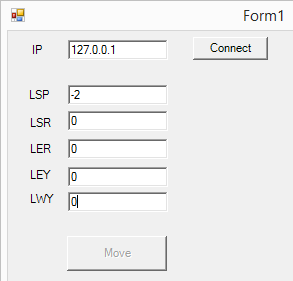
\includegraphics[scale=0.8]{Bilder/nao_prototyp1.PNG}
	\caption{Erster Nao-Prototyp}						
	\label{f:nao_prototyp1}						
\end{figure}
\noindent
In die anderen Felder müssen die einzelnen Winkel (im Bogenmaß) für die Gelenke (LSP = LeftShoulderPitch, LSR = LeftShoulderRoll, usw.) eingetragen werden. Bei Klick auf den Button \textit{Move} werden die einzelnen Winkel des linken Arms in die Position der eingetragenen Werte gefahren. In diesem Fall hebt der Roboter den linken Arm nach oben an, da \textit{LSP} mit -2rad definiert ist und dies im Nao-Gelenkraum einem Winkel von $-115^{\circ}$ entspricht (Siehe Kapitel \ref{tab:Lgelenkraum} und Abbildung \ref{f:gelenkraumL}). Ist ein angegebener Winkel nicht im Gelenkbereich wird die komplette Bewegung nicht ausgeführt (gilt nur für diesen Prototyp).

\subsection{Zweiter Prototyp}
Anhand der ersten Prototypen wurde das nun erworbene Wissen in eine gemeinsame Architektur eingebettet (Siehe \myref{k:Architektur}). Als Verbesserungen wurden alle benötigten Winkel auf zwei separaten Fenstern angezeigt, eines für jeden Arm. Auf der Fensteroberfläche wird nun das komplette Skelett über das RGB-Bild gelegt (siehe Abbildung \ref{f:programm}).


\subsection{Endprogramm}
Um den effektiven Algorithmus der Winkelerkennung noch effizienter zu gestalten, wurde noch ein Medianfilter implementiert, um die Ausreißer in den erkannten Winkeln zu eliminieren und somit die Messungenauigkeit der Gelenkpositionen zu verringern.
\newline
An der Oberfläche aus dem zweiten Prototyp wurde nicht mehr viel verändert. Lediglich eine Eingabemaske für die IP-Adresse des Nao-Roboters wurde hinzugefügt. Diese wird direkt bei Start des Programmes angezeigt.

\begin{figure}[H]						
	\centering							
	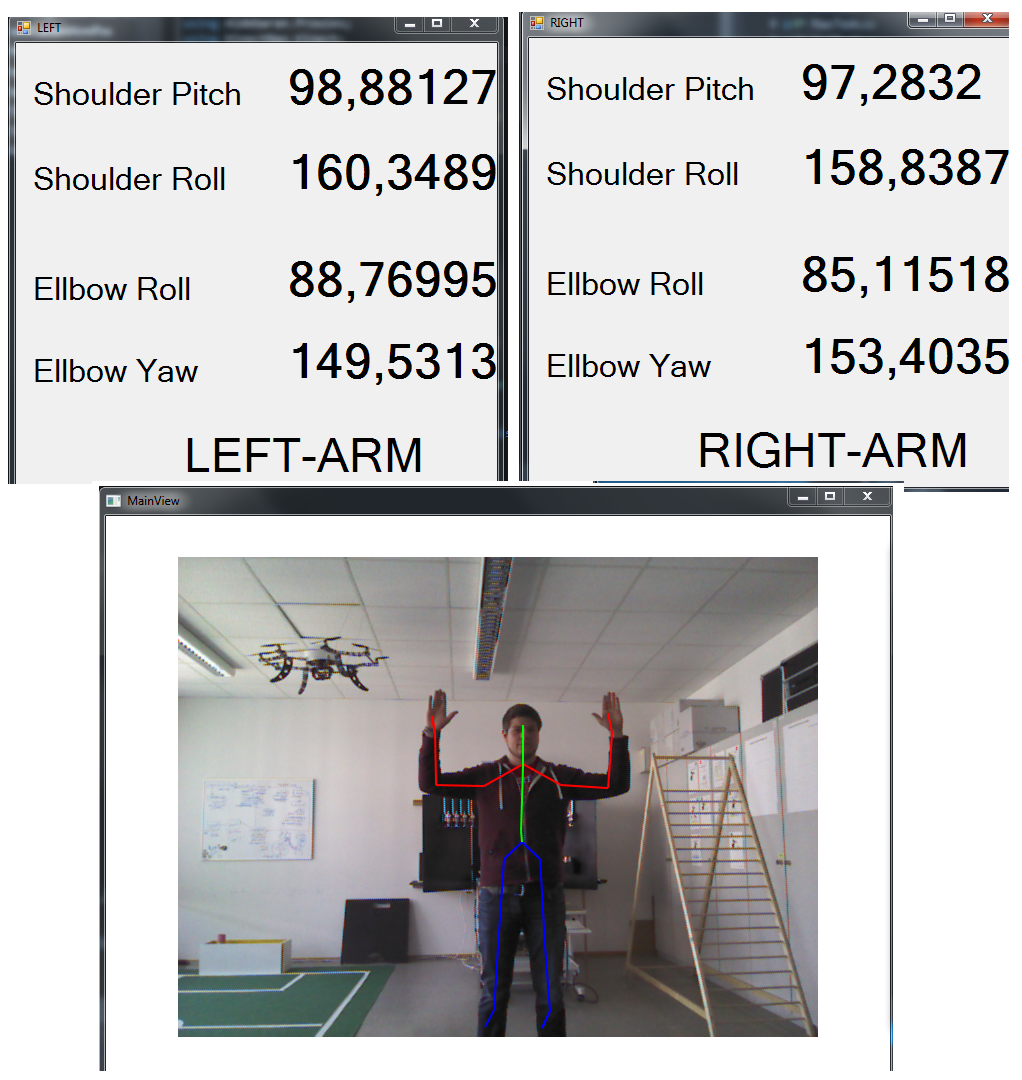
\includegraphics[scale=0.4]{Bilder/Programm.png}
	\caption{Fertige Applikation}						
	\label{f:programm}						
\end{figure}


%\todo{Screenshot von Prototypprogramm}

\chapter{Ausblick}      % Kapitelname
Schluss



%
% Sammlung aller aufgetretener Probleme während der Implementierung
%
%
%	Kinect Beendet nicht richtig
%		-> Eigene Klasse erstellt, die herunterfaehrt = Known Issue Microsoft
%
%
%
%	Ruckeln im Nao Arm
%		-> Kinect Filter (gleitender Mittelwertfilter über letzen 3 Werte)
%		-> Nao Speed geregelt (Geschw. zu den Winkeln)
%

\section{Aufgetretene Probleme}
\section{Weiterführende Anwendungsgebiete}
Es stellt sich nun die Frage, welchen technischen Nutzen die Teleoperation innerhalb der Gesellschaft finden könnte.
Zunächst gibt es ein großes Anwendungsgebiet in der Medizin....

%Medizin, Bombenentschärfung, leider auch Militär 
%
% 	Ausblick
%		Was koennte man noch machen?
%		Was koennte man verbessern?
%
%
%
%
\newpage

%\section*{Anhang}

        % Anhang Einbinden
%%%%%%%%%%%%%%%%%%%%%%%%%%%%%%%%%% Literaturverzeichnis %%%%%%%%%%%%%%%%%%%%%%%%%%%%%%%%%%%%%%%%%%%%%%%%%%%%%%%%%%%%%%%%%%%%%%%%%%%%%%%%%%%%%%%%%%%%%%%%%%%%%%%%%%%%%%%%%%
\addcontentsline{toc}{chapter}{Literaturverzeichnis}
\bibliographystyle{plain}        % Zitierformat (deutsch für Großschreibung) [Häufigkeit] im Text
\bibliography{Literaturverzeichnis}      % Pfad des Literaturverzeichnisses


% Das muss nach dem letzten \todo des gesamten Dokuments stehen
\todos                     % Liste der ToDo's --> Pakte: todo und Kommando \todo{..}

\end{document}  %%%%%%%%%%%%%%%%%%%%%%%%%%%%%%%%%%%%%%%%%%%%%%%%%%%%%%%%%%%%%%%%%%%%%%%%%%%%%%%%%%%%%%%%%%%%%%%%%%%%%%%%%%%%%%%%%%%%%%%%%%%%%%%%%%%%%%%%%%%%%%%%%%%%%%%%%%
